\documentclass{article}

% Language setting
% Replace `english' with e.g. `spanish' to change the document language
\usepackage[english]{babel}

% Set page size and margins
% Replace `letterpaper' with `a4paper' for UK/EU standard size
\usepackage[letterpaper,top=2cm,bottom=2cm,left=3cm,right=3cm,marginparwidth=1.75cm]{geometry}

% Useful packages
\usepackage{amsmath}
\usepackage{graphicx}
\usepackage[colorlinks=true, allcolors=blue]{hyperref}

\title{Lab 1}
\author{B12-224 - Nguyen Trung Kien}

\begin{document}
\maketitle

\section{Protocol}

\begin{figure}[h]
\centering
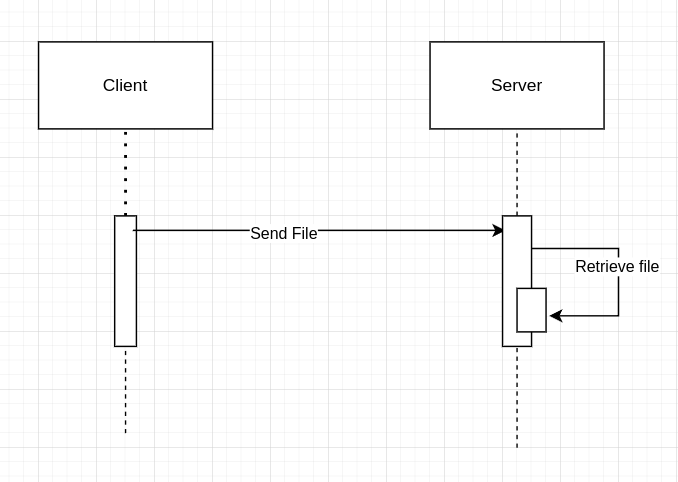
\includegraphics[width=0.8\linewidth]{Protocol.png}
\caption{\label{fig:Protocol}Protocol Design.}
\end{figure}

\section{System Organization}

\begin{figure}[h]
\centering
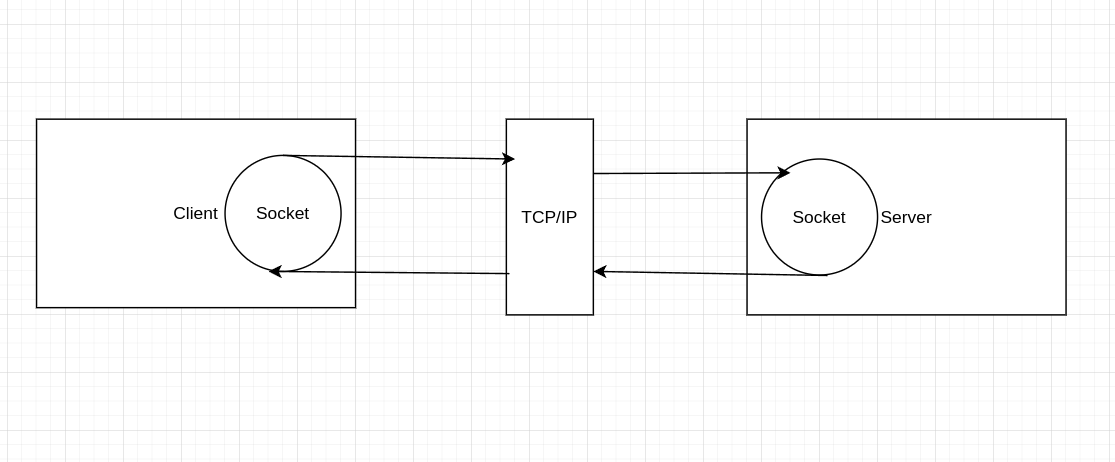
\includegraphics[width=0.8\linewidth]{System.png} % Adjust width here for a bigger picture
\caption{\label{fig:System}System architecture.}
\end{figure}

\section{File Transfer}
\subsection{Server Side (server.c)}
\begin{verbatim}
Include Header Files and Libraries: The server includes necessary header files like stdio.h, stdlib.h, sys/types.h, sys/socket.h, unistd.h, arpa/inet.h, and fcntl.h.
Define Constants: Constants like PORT and SIZE are defined.
Create Socket: The server creates a socket using socket() function, specifying AF_INET for IPv4 and SOCK_STREAM for TCP protocol.
Bind Socket: The server binds the socket to a specific port using bind() function.
Listen for Connections: It starts listening for incoming connections on the specified port using listen() function.
Accept Connection: When a client connects, the server accepts the connection using accept() function.
Open File: The server creates a file named received_file.txt in write-only mode using open() function.
Receive and Write Data: It receives data from the client using recv() function and writes it to the file using write() function.
Close File and Socket: After receiving and writing the data, the server closes the file and socket.
\end{verbatim}

\subsection{Client Side (client.c)}
\begin{verbatim}
Include Header Files and Libraries: The client includes necessary header files like stdio.h, stdlib.h, sys/types.h, sys/socket.h, unistd.h, arpa/inet.h, and fcntl.h.
Define Constants: Constants like PORT and SIZE are defined.
Create Socket: The client creates a socket using socket() function, specifying AF_INET for IPv4 and SOCK_STREAM for TCP protocol.
Establish Connection: It establishes a connection to the server using connect() function.
Open File: The client opens the file named sent_file.txt in read mode using fopen() function.
Read Data and Send to Server: It reads data from the file using fread() function and sends it to the server using write() function.
Close File and Socket: After the data transmission is complete, the client closes the file and socket.
\end{verbatim}

\subsection{Communication}
Both client and server communicate over the established TCP connection. The client reads data from the file and sends it to the server. The server receives the data and writes it to the specified file.

\end{document}
